\chapter{Some observations concerning passing electrons}
\vspace*{3mm}
Many generalisations of the \AE{} calculation are possible, and all depend {\it critically} on the chosen invariants, and different choices of invariants have been considered before. The following chapter considers an especially natural generalisation of the results in the current thesis, by investigating passing electrons, and I am grateful for both P. Helander and E. Rodr\'iguez for providing crucial insights here. The generalisation is included, as the calculation of the \AE{} is entirely equivalent with only minor interpretative differences.

\section{Invariants on other species}
We have seen in the past publication that the \AE{} of trapped electrons serves as a useful measure of gyrokinetic turbulence. Though the research is fruitful, it is lacking in some parts: ions are not accounted for, nor are passing electrons. It is thus natural to wonder if the \AE{} may be extended to account for these species. One such investigation is presented in \citet{helander2020available}, where the following assumptions are put forth concerning the various species:
\begin{itemize}
    \item All species obey Liouville's theorem.
    \item The trapped electrons have invariance of $\mu$ and $\mathcal{J}$.
    \item The ions have invariance of $\mu$ alone.
    \item Passing electrons have invariance of $\mu$ and $\psi$.
    \item The electron and ion densities are quasineutral, i.e. the ion charge density exactly balances the electron charge density.
\end{itemize}
Invariance of $\psi$ of passing electrons is motivated by the fast streaming of the electrons, which ensures that the radial drift vanishes to leading order on irrational surfaces \cite{helander2014theory}. This constraint is, however, especially restrictive as invariance of $\psi$ renders it impossible extract energy via flattening of the gradient and the \AE{} vanishes exactly. We know, however, that there may be situations where passing electrons can contribute to various instabilities \cite{jenko2000electron,landreman2015universal,helander2015universal,hardman2022extended,costello2022universal}. Let us somewhat weaken the assumptions imposed on these passing electrons, and there is an especially natural choice one can make which extends naturally the research presented in this thesis. 

\subsection*{An equivalent $\mathcal{J}$ for passing particles}
Let us return to Eq. \eqref{eq: euler-lagrange for psi}, the Euler-Lagrange equation for the radial coordinate. Restating the result for convenience, we had found the following relationship
\begin{equation}
    \frac{\mathrm{d}}{\mathrm{d}t}\left( \psi + \frac{m \dot{\ell}}{q} \boldsymbol{b} \cdot \partial_\alpha \boldsymbol{R} \right) = - \frac{\mu}{q} \partial_\alpha B.
\end{equation}
By integrating between two bounce-points (where $\dot{\ell}$ vanishes), we were able to relate the total radial excursion a trapped particle makes to derivatives of $\mathcal{J}$. Let us now instead consider a passing particle, in a periodic domain (as may be found in a tokamak, or on a rational surface of a stellarator), and we integrate across this domain. Due to this periodicity, we have that
\begin{equation}
    \int_{\rm period} \frac{\mathrm{d}}{\mathrm{d}t} \left( \frac{m \dot{\ell}}{q} \boldsymbol{b} \cdot \partial_\alpha \boldsymbol{R} \right) \mathrm{d} t = 0,
\end{equation}
and, using $E = \mu B + m v_\parallel^2/2$, the Euler-Lagrange equation becomes
\begin{equation}
    q\Delta \psi = \partial_\alpha \int_{\rm period} m v_\parallel \mathrm{d} \ell \equiv \partial_\alpha \mathcal{J}_{p}.
\end{equation}
We have thus found that a passing equivalent of $\mathcal{J}$ behaves entirely analogously to the trapped one. For the binormal coordinate, one finds
\begin{equation}
    q\Delta \alpha = - \partial_\psi \mathcal{J}_p,
\end{equation}
and one again finds that the differential $\mathrm{d}\mathcal{J}_p = 0$, showcasing its invariance. \par 
It is thus a natural choice to impose that $\mu$ and $\mathcal{J}_p$ are conserved for these passing particles, and the calculation of the \AE{} is completely equivalent to the one presented for trapped particles. The only interpretative difference is that $\omega_\alpha$ and $\omega_\psi$ now refer to the radial and binormal drift \textit{passing} particles experience in one transit of the domain, where the transit time is given by $\partial_E \mathcal{J}_p$. This equivalence similarly implies that the stabilising properties of maximum-$\mathcal{J}_p$ transfer to the passing population, too. Since $\partial_\alpha \mathcal{J}_p \propto \omega_\psi$ is often much reduced (if not zero) for these passing particles, let us focus on the behaviour of $\partial_\psi \mathcal{J}_p$ of these passing particles.

\section{The maximum-$\mathcal{J}_p$ property}
The analysis of the binormal drift of passing particles is made simpler due to the fact that the singular behaviour bounce-averaging integrals exhibit is not present for passing particles. As such, we may simply investigate the expression for the passing adiabatic invariant and take derivatives without further complications. The passing invariant may be written as
\begin{equation}
    \mathcal{J}_p = \sqrt{2 m E }  \int_{\rm period} \sqrt{1 - \lambda \hat{B}} \: \mathrm{d} \ell,
\end{equation}
with $\lambda = \mu B_0/ E$, $B_0$ is some reference magnetic field, and $\hat{B} = B/B_0$. Taking the derivative with respect to $\psi$, one finds
\begin{equation}
    \partial_\psi \mathcal{J}_p = - \sqrt{\frac{m E}{2}} \int_{\rm period} \frac{\lambda \partial_\psi \hat{B}}{\sqrt{1 - \lambda \hat{B}}} \mathrm{d} \ell.
\end{equation}
The derivative with respect to $E$ may similarly be found as
\begin{equation}
    \left( \partial_E \mathcal{J}_p \right)_{\psi,\alpha,\mu} = \sqrt{\frac{m}{2E}} \int_{\rm period} \frac{\mathrm{d} \ell}{\sqrt{1 - \lambda \hat{B}}},
\end{equation}
and the binormal drift hence reduces to
\begin{equation}
    \omega_\alpha = \frac{E}{q} \frac{\int_{\rm period} (1 - \lambda \hat{B})^{-1/2} \lambda \partial_\psi \hat{B} \: \mathrm{d} \ell }{\int_{\rm period} (1 - \lambda \hat{B})^{-1/2} \: \mathrm{d} \ell}.
\end{equation}
We are now in a position to evaluate the drift. Realize that passing particles have $\lambda \in [0,\hat{B}_{\rm  max}^{-1})$, and it is natural to consider the two limiting cases. For purely passing particles (i.e. $\lambda \rightarrow 0$), we find the leading order expression
\begin{equation}
    \omega_\alpha (\lambda \rightarrow 0) \approx \frac{\lambda E}{q} \frac{\int_{\rm period} \hat{B} \partial_\psi \hat{B} \: \frac{\mathrm{d} \ell}{\hat{B}} }{\int_{\rm period} \hat{B} \: \frac{\mathrm{d} \ell}{\hat{B}}} \approx \frac{\lambda E}{2q} \frac{\langle \partial_\psi \hat{B}^2 \rangle_{\rm fs}}{\langle\hat{B} \rangle_{\rm fs}},
\end{equation}
where we have introduced the flux-surface averaging operator as $\langle \dots \rangle_{\rm fs}$. The above expression is similar to the \textit{magnetic well} term, useful for determining magnetohydrodynamic stability \cite{greene1997brief,landreman2020magnetic,rodriguez2023magnetohydrodynamic}. For favorable magnetodhydrodynamic stability properties, one requires that $D_{\rm well} \propto \langle \partial_\psi \ln \hat{B} \rangle_{\rm fs} > 0$ \cite{helander2014theory}. The maximum-$\mathcal{J}_p$ property requires that $q \omega_\alpha >0 \implies \langle \partial_\psi \hat{B}^2 \rangle_{\rm fs} > 0$, and we thus see a correspondence between the magnetic well and maximum-$\mathcal{J}$ property. More precisely, if one expands $\hat{B}$ around smallness in its variation, the criteria to leading order are equivalent, and there is thus a synergy between this magnetohydrodynamic stability criterion and the maximum-$\mathcal{J}_p$ property for passing particles. \par 
Let us next investigate a second limiting case, namely the barely passing particles which have $\lambda \rightarrow \hat{B}_{\rm  max}^{-1}$. Such passing particles spend all their orbit-time near the global maximum of $B$ on the flux surface, and as such sample $\partial_\psi B$ only at this location. Denote $\hat{B}(\ell_{\rm max}) = \hat{B}_{\rm max}$, we then have that
\begin{equation}
    q \omega_\alpha (\lambda \rightarrow \hat{B}_{\rm  max}^{-1}) = \frac{E}{\hat{B}_{\rm max}} \partial_\psi \hat{B}(\ell_{\rm max}).
\end{equation}
To investigate the sign of $\partial_\psi B(\ell_{\rm max})$, let us consider the following. 
\begin{enumerate}
    \item Assume that $\partial_\psi B(\ell_{\rm max}) < 0 $ for all $\psi$. This implies that there is a point-maximum in $B$, somewhere on the magnetic axis. However such a point-maximum  is impossible as a consequence of Earnshaw's theorem \cite{earnshaw1848nature}, and near the magnetic axis one {\it must} have that $\partial_\psi B(\ell_{\rm max}) > 0$.
    \item Let us next assume that $B_{\rm max}$ is unique on the flux surface (this excludes, for example, exactly omnigeneous equilibria). If we then assume that $\partial_\psi B(\ell_{\rm max})$ changes sign for some $\psi > 0$, we have again introduced a local point maximum at the point $\partial_\psi B = 0$. This is once again impossible due to Earnshaw's theorem, and as such we find that $\partial_\psi B > 0 $. If we instead assume that $B_{\rm max}$ is not unique but there is a line of constant $B_{\rm max}$, one simply has one ignorable coordinate and Earnshaw's theorem still holds. So, in this case too, barely passing particles are maximum-$\mathcal{J}_p$.\footnote{I wish to stress that this crucial insight was provided to me by Helander and Rodriguez for which I am thankful, and this finding proved crucial in their investigation of the maximum-$\mathcal{J}$ property in quasi-isodynamic systems which will be published soon.}
\end{enumerate}
We have thus found that the barely passing particles are in all scenarios maximum-$\mathcal{J}_p$. \par 
All in all we have investigated two limiting cases. Purely passing particles are maximum-$\mathcal{J}_p$ if the flux-surface average of $\partial_\psi B^2$ is greater than zero (similar to the magnetic well), and barely passing particles are maximum-$\mathcal{J}_p$ due to the impossibility of point-maxima in $B$. Let us then postulate that, if both limiting cases are maximum-$\mathcal{J}_p$, they are connected monotonically in $\lambda$ and thus all particles are maximum-$\mathcal{J}_p$.

\subsection*{An example case: the large-aspect ratio limit}
Let us, as an example case showcasing our findings of the previous section, calculate the drift in a large-aspect-ratio tokamak with circular flux-surfaces. In such a limit, we know that the arc-length relates the the geometric poloidal angle $\theta$ via $\mathrm{d}\ell \approx R_0 \mathrm{d} \theta / \iota$, and the magnetic field is $\hat{B} \approx 1 - \frac{r}{R_0} \cos \theta$ \cite{helander2005collisional}. The passing invariant thus becomes
\begin{equation}
    \mathcal{J}_p \approx \frac{R_0}{\iota} \sqrt{2mE} \int_{-\pi}^{\pi} \sqrt{1 - \lambda (1 - \epsilon\cos \theta)} \: \mathrm{d} \theta,
\end{equation}
where we have introduced $\epsilon = r/R_0$. We may readily take derivatives with respect to $\epsilon$ and $H$ to find the drift, and the result to leading order in smallness of $\epsilon$ is
\begin{equation}
    q \omega_\alpha = \frac{H}{B_0 R_0 r} \left(\frac{2}{k^2} \left[1 - \frac{E(k)}{K(k)} \right] - 1 \right) \equiv \frac{H}{B_0 R_0 r} \mathcal{F}(k).
\end{equation}
Here we have defined the ``passing'' parameter as $k^2 = 2 \lambda \epsilon / ( 1 + \lambda [ \epsilon - 1 ] )$, which is zero for purely passing particles and one for barely trapped particles. Furthermore, the complete elliptic integrals of the first and second kind are defined as $K(k) = \int_{-\pi}^{\pi} (1 - k^2 \sin^2 \theta)^{-1/2} \mathrm{d} \theta$ and $E(k) = \int_{-\pi}^{\pi} (1 - k^2 \sin^2 \theta)^{1/2} \mathrm{d} \theta$. \par 
In terms of the previous section, we find that for around $k^2$ the drift goes as $\mathcal{F}(k \rightarrow 0) \approx k^2 / 8$. For barely passing particles one finds $\mathcal{F}(1) = 1$, and intermediate values are included in the plot of $\mathcal{F}(k)$ given in Fig. \ref{fig: F(k)}. For the case given here it can be seen that all particles are indeed maximum-$\mathcal{J}_p$.
\begin{figure}
    \centering
    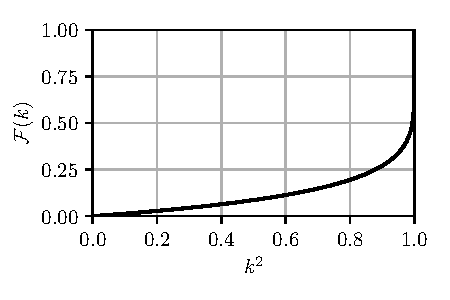
\includegraphics[width=0.6\textwidth]{3_chapters/2_conclusion_outlook/Fk.pdf}
    \caption{The passing particle drift as a function of the parameter $k$.}
    \label{fig: F(k)}
\end{figure}

\section{When is conservation of $\mathcal{J}_p$ relevant?}
Finally, let us consider under what conditions invariance of $\mathcal{J}_p$ is relevant for turbulent transport. The particles should reside in the domain long enough, so that turbulence may substantially reorder particles and one may reach a state akin to a ground-state. To be somewhat more precise, the typical residence time of a passing particle in a domain where turbulence resides should be at comparable or greater than typical drift-wave turbulence time-scales. Evidently, irrational surfaces break such criteria as particles sample different field-lines with different turbulent structures on it after each transit. Hence a minimal condition one should meet is that the flux-surface should be a, preferably low-order, rational surface. In order to ensure that neighboring surfaces also meet such properties so that the turbulence may flatten gradients across surfaces, the magnetic shear should similarly not be too large. From the discussion and example given in the preceding sections we have postulated that most equilibria satisfy the maximum-$\mathcal{J}_p$ condition, implying stabilising properties of such low-shear rational surfaces. Such surfaces are often found to be regions where internal transport barriers show up, which are regions with much reduced transport and increased gradients \cite{fujita1997internal,turri2008role,ida2018internal}, though it should be noted that $\boldsymbol{E} \times \boldsymbol{B}$-shearing is thought to play an important role here which the current theory does not account for. \par 
All in all, the above gives a straightfoward method of generalizing the results in the rest of the thesis to account for passing electrons, with some observations of possible use-cases, using the same tools employed in the rest of the thesis. There is, of course, reasons to be sceptical of possible success of this method. Firstly, one should not expect to accurately model electron-temperature-gradient mode driven turbulence with this method, as both the transit time of the passing electrons and the bounce time of trapped electrons becomes comparable with the typical turbulence timescales. Hence, only in trapped electron mode or ion temperature gradient mode driven scenarios should one expect this measure to be reliable.
